\documentclass[11pt]{beamer}
%Gummi|061|=)
\usepackage[italian]{babel}
\usepackage[utf8x]{inputenc}
\usepackage{hyperref}
\usepackage{graphicx}
\usepackage{amsmath}
\usepackage{xcolor}
\DeclareMathOperator{\Tr}{Tr}
\DeclareMathOperator{\Exp}{exp}
\DeclareMathOperator{\Log}{log}
\DeclareMathOperator{\Det}{det}

\newsavebox\MBox
\newcommand\Cline[2][red]{{\sbox\MBox{$#2$}%
  \rlap{\usebox\MBox}\color{#1}\rule[-1.2\dp\MBox]{\wd\MBox}{0.5pt}}}

\title{\textbf{Tecniche combinatorie nel Modello di Ising bidimensionale}}
\author{Alberto Botto Poala \\
Relatore Prof. Marco Billò}
\date{14.04.2014}

\begin{document}

\begin{frame}
 \maketitle
\end{frame}

\begin{frame}
	\frametitle{Evidenze Sperimentali}
Un atomo può essere dotato di un piccolissimo momento magnetico per due motivi
	\begin{itemize}
	\item{rotazione degli elettroni attorno al nucleo}
	\item{spin degli elettroni}
 	\end{itemize}
Momento magnetico totale $\to$ somma dei due momenti.\\
\center{\textbf{ATOMO $\approx$ PICCOLA CALAMITA}}
	\begin{figure}[h]
	\centering
	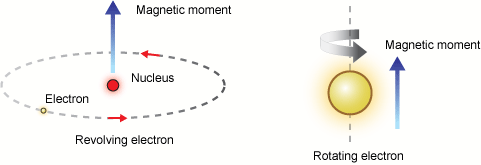
\includegraphics[width=0.9\columnwidth]{pt2}

	\label{fig1}
	\end{figure}
\end{frame}

\begin{frame}
	\frametitle{Evidenze Sperimentali}
Possono queste piccole calamite allinearsi e dare vita ad un campo magnetico sensibilmente più grande? 
\center{\textbf{PARAMAGNETISMO}$ \ \rightarrow \ \leftarrow \ $\textbf{FERROMAGNETISMO}}


\begin{figure}[r]
	\centering
	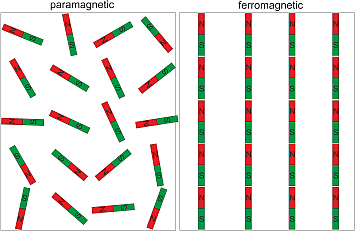
\includegraphics[width=0.6\columnwidth]{pt1}
		\label{fig1}
	\end{figure}

\end{frame}

\begin{frame}
	\frametitle{Evidenze Sperimentali}
Questa  \textbf{transizione di fase} avviene
\begin{itemize}
\item<1->{ ad una specifica temperatura $T_C$, detta temperatura di Curie}
\item<2->{Per $T<T_C$ vi è allineamento.\\
La suscettività magnetica segue la legge di Curie-Weiss
$$ \chi_m = \frac{C \rho}{T-T_C} $$
con $C$ costante del materiale e $\rho$ la sua densità.
}
\item<3->{Per $T>T_C$ non vi è alcun allineamento}
\item<4->{\textbf{Il Modello di Ising nasce per studiare la dinamica di questo allineamento}}
\end{itemize}
\end{frame}

\begin{frame}
	\frametitle{Storia del Modello di Ising}
Il problema del ferromagnetismo può essere formulato in una, due o tre dimensioni (o più).
	\begin{itemize}
	\item{\textbf{1-D} Catena monodimensionale periodica di atomi, studiata da Ernst Ising nel 1924, sotto la guida di Wilhelm Lenz.}
	\end{itemize}
	\begin{figure}[r]
	\centering
	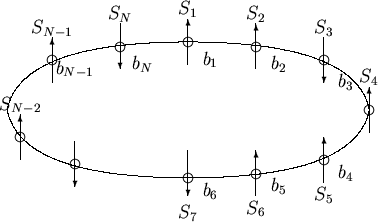
\includegraphics[width=0.6\columnwidth]{pt3}

	\label{fig1}
	\end{figure}
	

\end{frame}

\begin{frame}
	\frametitle{Storia del Modello di Ising}
\begin{itemize}
\item<1->{La soluzione monodimensionale non presenta transizioni di fase. 
	\begin{figure}[r]
	\centering
	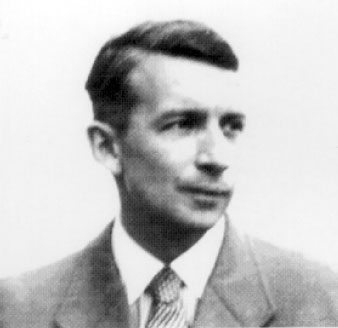
\includegraphics[width=0.2\columnwidth]{pt4}
	\caption{Ernst Ising 1900-1998}
	\label{fig1}
	\end{figure}
	}
	\item<2->{Ising riteneva che anche in più dimensioni non ci sarebbero state transizioni di fase. (cfr. \emph{Beitrag zur Theorie des
Ferro - und Paramagnetismus}, 1924, BIBLIOTHECA AUGUSTANA on line)}
\end{itemize}
\end{frame}
	
\begin{frame}
	\begin{itemize}
	\frametitle{Storia del Modello di Ising}
 	\item{\textbf{2-D} Reticolo di atomi. Venne risolta nel 1949 da Lars Onsager. Già in due dimensioni il modello mostra delle transizioni di fase.}
 	\begin{figure}[r]
	\centering
	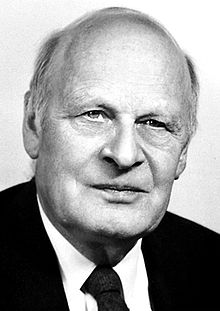
\includegraphics[width=0.2\columnwidth]{pt5}
	\caption{Lars Onsager 1903-1976}
	\label{fig1}
	\end{figure}
 	\item{\textbf{3-D} Esistono simulazioni numeriche ma la soluzione analitica non è ancora stata trovata}
 	\end{itemize}
 \end{frame}
 \begin{frame}
 \frametitle{Modello di Ising - Soluzione di Vdovichenko}
\center{Cosa vedremo} 
\begin{itemize}
\item<1->{Solo Modello \textbf{2-D}}
\item<2->{Sviluppo alta temperatura per \textbf{$Z(T)$}}
\item<3->{Soluzione combinatoria di Vdovichenko per \textbf{$F(T)$}}
\end{itemize}

\end{frame}

\begin{frame}
 \frametitle{Il Reticolo}
Reticolo quadrato periodico con $L\times L=N$ siti.
\begin{figure}[r]
	\centering
	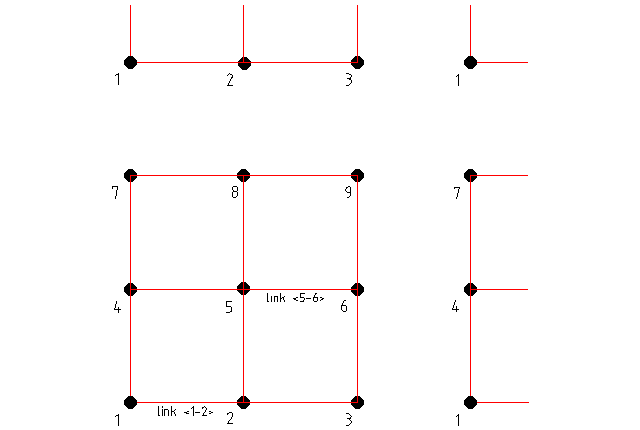
\includegraphics[width=0.55\columnwidth]{ret33}
	\caption{Reticolo periodico $3\times3$}
	\label{fig1}
	\end{figure}
	\begin{itemize}
	\item<1->{atomo $\to$ sito}
	\item<2->{sito $i$-esimo $\to \sigma_i=\pm1$ (oppure spin $\uparrow$ o $\downarrow$). Rappresenta il momento magnetico.}
	\item<3->{Scelta dell'interazione $\to$ Scelta dell'Hamiltoniana}
	\end{itemize}
\end{frame}
 
  \begin{frame}
 \frametitle{Approssimazioni}
 \center{Interazione solo tra i primi vicini. La connessione è detta \textbf{Link}.}
 \begin{figure}[r]
	\centering
	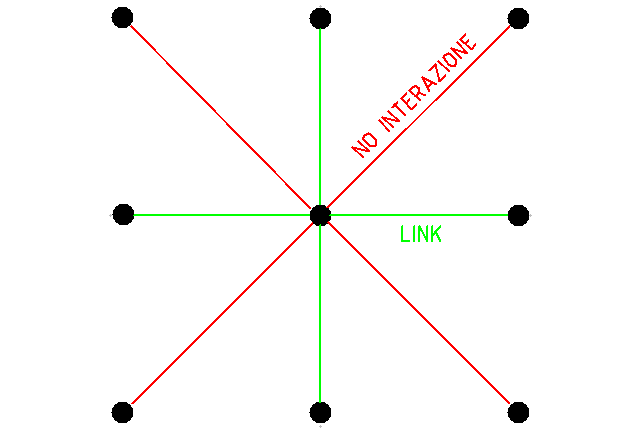
\includegraphics[width=0.7\columnwidth]{appr}
	\caption{Schema delle interazioni}
	\label{fig1}
	\end{figure}
\end{frame}
 
 \begin{frame}
 \frametitle{Funzione di Partizione nell'Ensemble Canonico}
Scelta l'\textbf{Hamiltoniana} 
 $$H_N=-J\sum_{(i,j)}\sigma_i\sigma_j-J'\sum_{(i,k)}\sigma_i\sigma_k
 $$
 e nota la definizone della \textbf{Funzione di Partizione} per l'Ensemble Canonico 
 $$\sum_\sigma e^{-\beta E_\sigma}
 $$
 con $\sigma= \{ \sigma_1,\sigma_2...\sigma_N \} $, si giunge facilmente alla Funzione di Partizione del nostro modello
 $$
 Z_N=\sum_\sigma \exp[\beta J\sum_{(i,j)}\sigma_i\sigma_j+\beta J'\sum_{(i,k)}\sigma_i\sigma_k]
 $$
\end{frame}

\begin{frame}
\frametitle{Sviluppo ad Alte Temperature}
Si può manipolare questa espressione e ottenere
$$
Z_N=(\cosh{K}\cosh{K'})^N\sum_{\sigma}\left(\prod_{(i,j)}(1+v\sigma_i\sigma_j)\prod_{(i,k)}(1+w\sigma_i\sigma_k)\right) 
$$
$$
\mbox{con \ } \begin{cases} \  v=\tanh{J/kT}=\tanh{K} \\  \ w=\tanh{J'/kT}=\tanh{K'}
\end{cases}
$$
Notiamo che
$v$, $w<1 \ \forall T \to$ \textbf{sviluppo in serie}

\center{Cosa vuol dire sviluppare in serie $Z_N$ in $v$ e $w$?}
\end{frame}
\begin{frame}
	\frametitle{Sviluppo ad Alte Temperature}
Esplicitiamo
	\begin{equation}
	\begin{split}
&\prod_{(i,j)}(1+v\sigma_i\sigma_j)\prod_{(i,k)}(1+w\sigma_i\sigma_k)=\\ 
&(1+v\sigma_1\sigma_2)\times(1+v\sigma_2\sigma_3)\times...\times(1+v\sigma_{N-1}\sigma_{N})... \\ & \times(1+w\sigma_1\sigma_{L+1})\times(1+w\sigma_2\sigma_{L+2})\times...\times(1+v\sigma_{L(L-1)}\sigma_{N})
	\end{split}
	\end{equation}
	Che cosa ottengo?
	\begin{itemize}
	\item{1}
	\item{$v\sigma_i\sigma_{i+1} $ e $ w\sigma_j\sigma_{L+j}$}
	\item{prodotti dei precedenti. \\
	Esempio (reticolo $4\times4$):
$$(v\sigma_{5}\sigma_{6})(v\sigma_{6}\sigma_{7})(v\sigma_{11}\sigma_{12})(w\sigma_{1}\sigma_{5})(w\sigma_{10}\sigma_{14})
$$ }
	\end{itemize}
\end{frame}


\begin{frame}
\frametitle{Configurazione grafica sul reticolo}
 Questi termini analitici hanno anche un significato geometrico.\\

Ogni termine può essere disegnato sul reticolo evidenziando i link che contiene. Cosa vuol dire? \\
Esempio precedente
$$(v\sigma_{5}\sigma_{6})(v\sigma_{6}\sigma_{7})(v\sigma_{11}\sigma_{12})(w\sigma_{1}\sigma_{5})(w\sigma_{10}\sigma_{14})
$$
\begin{figure}[r]
	\centering
	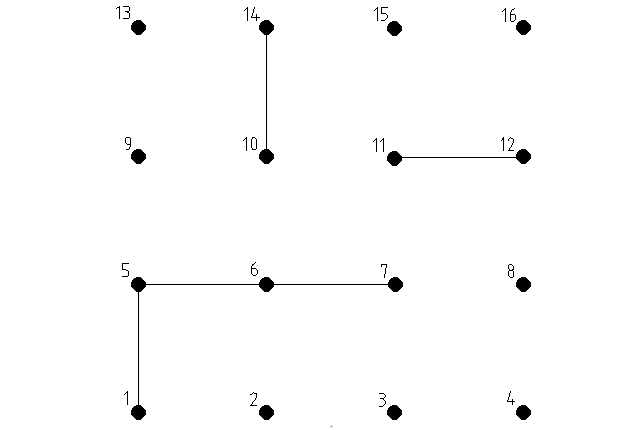
\includegraphics[width=0.5\columnwidth]{sat21}
	\caption{Configurazione grafica sul reticolo}
	\label{fig1}
	\end{figure}
\end{frame}

\begin{frame}
\frametitle{Configurazione grafica sul reticolo}
Altro esempio più interessante
$$(v\sigma_{1}\sigma_{2})(v\sigma_{5}\sigma_{6})(v\sigma_{6}\sigma_{7})(v\sigma_{10}\sigma_{11})(w\sigma_{1}\sigma_{5})(w\sigma_{2}\sigma_{6})(w\sigma_{6}\sigma_{10})(w\sigma_{7}\sigma_{11})
$$
\begin{figure}[r]
	\centering
	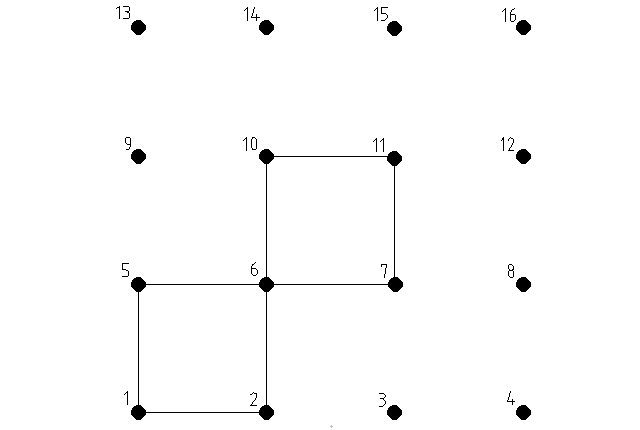
\includegraphics[width=0.5\columnwidth]{sat22}
	\caption{Configurazione grafica sul reticolo}
	\label{fig1}
	\end{figure}
$$
\mbox{Notiamo che \ } \begin{cases} \# \ v & \mbox{numero  di  link  orizzontali} \\ \# \ w & \mbox{numero di link verticali}
\end{cases}
$$

\end{frame}
	

 

\begin{frame}
\frametitle{Simmetrie in Z(T)}
Perchè l'esempio appena visto è più interessante?\\
\begin{itemize}
\item<1->{Ogni termine si può scrivere come
$$v^rw^s\sigma_1^{n_1}\sigma_2^{n_2}\sigma_3^{n_3}...
$$}
\item<2->{Non dimentichiamoci che
$$Z_N=(\cosh{K}\cosh{K'})^N\sum_{\sigma}\left(\prod_{(i,j)}(1+v\sigma_i\sigma_j)\prod_{(i,k)}(1+w\sigma_i\sigma_k)\right) 
$$}
\item<3->{Se $n_i$ dispari allora si cancella.}
\item<4->{$n_i$ numero di volte che tocco il sito $i$-esimo $\to$ sopravvivono solo i grafici chiusi. }
\end{itemize}
\end{frame}
\begin{frame}
\frametitle{Esempio di antisimmetria}
Primo esempio
$$(v\sigma_{5}\sigma_{6})(v\sigma_{6}\sigma_{7})(v\sigma_{11}\sigma_{12})(w\sigma_{1}\sigma_{5})(w\sigma_{10}\sigma_{14})=
$$
$$
=v^3w^2\sigma_1\sigma_{5}^2\sigma_{6}^2\sigma_{7}\sigma_{10}\sigma_{11}\sigma_{12}\sigma_{14}
$$

\begin{figure}[r]
	\centering
	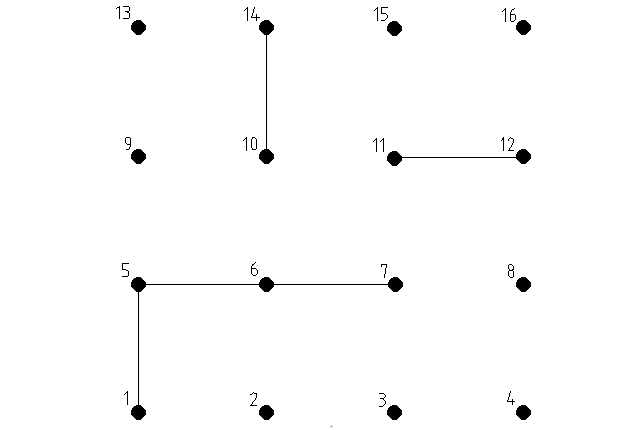
\includegraphics[width=0.5\columnwidth]{sat21}
	\caption{Configurazione grafica sul reticolo}
	\label{fig1}
	\end{figure}

\end{frame}

\begin{frame}
\frametitle{Esempio di simmetria}
Secondo esempio
$$(v\sigma_{1}\sigma_{2})(v\sigma_{5}\sigma_{6})(v\sigma_{6}\sigma_{7})(v\sigma_{10}\sigma_{11})(w\sigma_{1}\sigma_{5})(w\sigma_{2}\sigma_{6})(w\sigma_{6}\sigma_{10})(w\sigma_{7}\sigma_{11})=
$$
$$
=v^4w^4\sigma_1^2\sigma_{2}^2\sigma_{5}^2\sigma_{6}^4\sigma_{7}^2\sigma_{10}^2\sigma_{11}^2
$$

\begin{figure}[r]
	\centering
	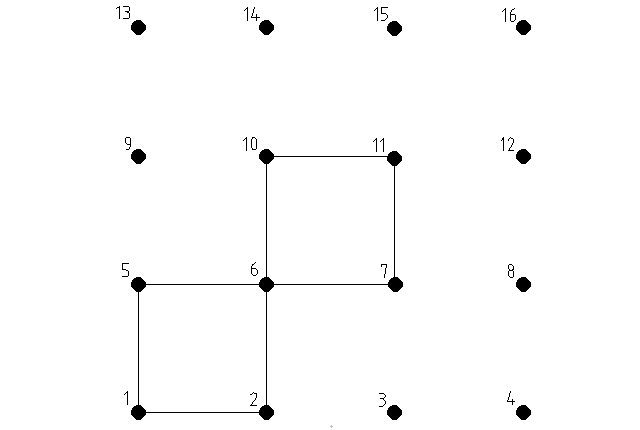
\includegraphics[width=0.5\columnwidth]{sat22}
	\caption{Configurazione grafica sul reticolo}
	\label{fig1}
	\end{figure}

\end{frame}

\begin{frame}
Sopravvivono solo i termini con $\sigma_i$ pari, quindi possiamo scrivere
$$v^rw^s\sigma_1^{n_1}\sigma_2^{n_2}\sigma_3^{n_3}...=v^rw^s
$$
Ne avremo $2^N$ per ogni valore della coppia $r$, $s$.\\
La funzione di partizione diventa
$$Z_N=2^N(\cosh{K}\cosh{K'})^N\sum_Pv^rw^s
$$
con $P$ insieme delle poligonali chiuse disgiunte.\\
Quindi com'è fatta $\Phi(v,w)=\sum_Pv^rw^s$?
\end{frame}

\begin{frame}
\frametitle{I primi termini dello sviluppo}
	\begin{equation}
	\begin{split}
\sum_Pv^rw^s=&1+\Cline[green]{Nv^2w^2}+\Cline{Nv^2w^4+Nv^4w^2}+\\
& +\Cline[blue]{Nv^2w^6+Nv^6w^2}+\frac{1}{2}N(N+5)v^4w^4+...
	\end{split}
	\end{equation}
	\begin{figure}[r]
	\centering
	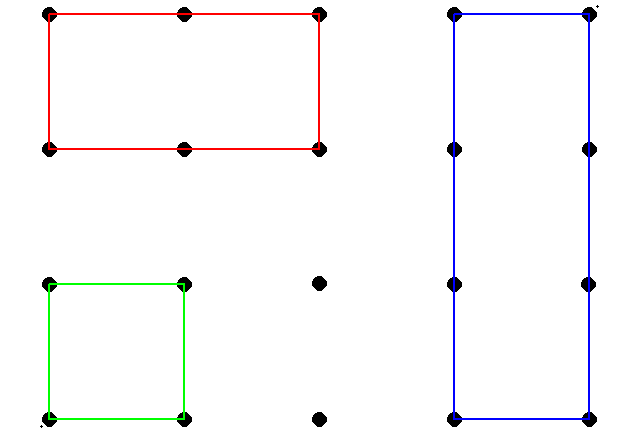
\includegraphics[width=0.55\columnwidth]{sviluppo}
	\caption{Configurazione grafica dei primi termini dello sviluppo}
	\label{fig1}
	\end{figure}


\end{frame}
\begin{frame}
\frametitle{I termini successivi}

I termini $\frac{1}{2}N(N+5)v^4w^4$ sono 

\begin{figure}[r]
	\centering
	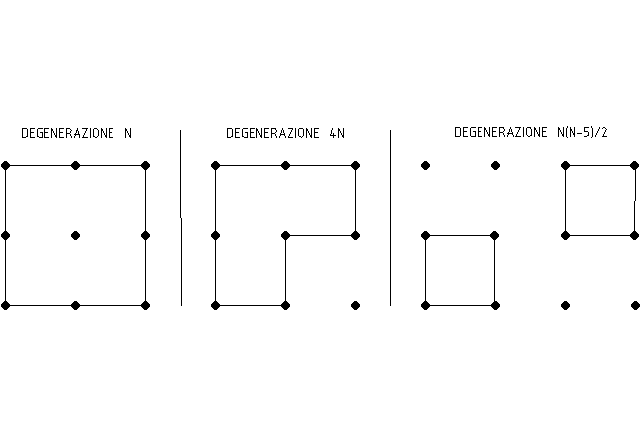
\includegraphics[width=0.8\columnwidth]{degenerazione}
	\caption{Configurazione grafica sul reticolo dei termini $v^4w^4$}
	\label{fig1}
	\end{figure}

	\end{frame}




\begin{frame}
\frametitle{Dallo sviluppo alla soluzione di Vdovichenko}
\begin{itemize}
\item{Abbiamo ottenuto lo sviluppo ad alte $T$ per la Funzione di Partizione $Z(T)$}
\item{Partiamo quindi con la \textbf{Soluzione combinatoria di Vdovichenko} per arrivare all'Energia Libera $F(T)$}
\end{itemize}
\end{frame}
\begin{frame}
Poniamo $J=J' \to v=w$.

	\begin{equation}
	\begin{split}
\Phi(v,w)=&1+\Cline[green]{Nv^2w^2}+\Cline{Nv^2w^4+Nv^4w^2}+\\
& +\Cline[blue]{Nv^2w^6+Nv^6w^2+\frac{1}{2}N(N+5)v^4w^4}+...=\\&
=1+\Cline[green]{Nv^4}+\Cline{2Nv^6}+\Cline[blue]{\frac{1}{2}N(N+9)v^8}...=\Phi(v)
	\end{split}
	\end{equation}
Anche la funzione di partizione si semplifica e diventa
\begin{equation}
Z_N=2^N(1-v^2)^{-N}\Phi(v)
\end{equation}
con
$$\Phi(v)= \sum_r g_r v^r
$$
L'unica incognita è $g_r$, numero di grafici disgiunti di perimetro $r$.\\

\end{frame} 


\begin{frame}
\frametitle{Dalle configurazioni grafiche ai cammini chiusi}
La soluzione di Vdovichenko prevede di trasformare le configurazioni grafiche come dei \textbf{cammini chiusi}.\\
Sorgono dei problemi:

\begin{figure}[r]
	\centering
	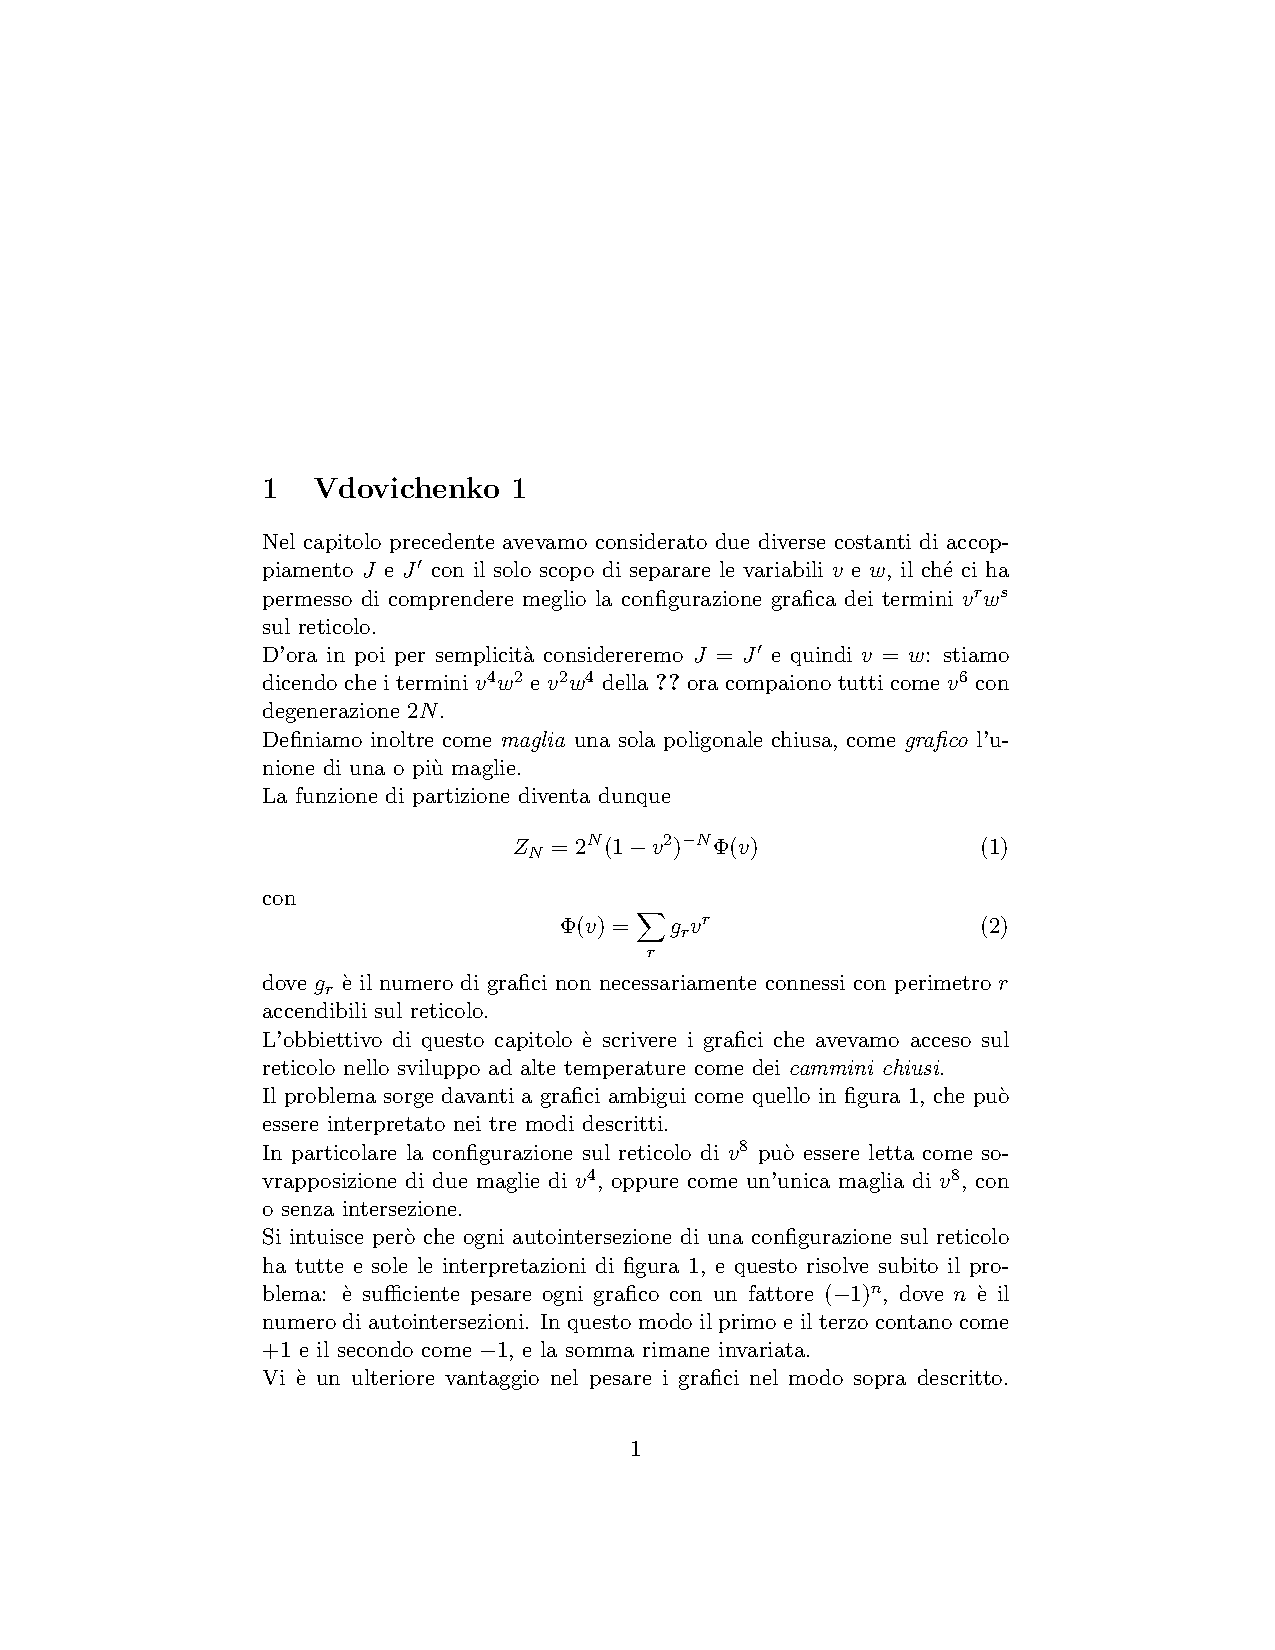
\includegraphics[width=0.6\columnwidth]{v1}
	\caption{Elemento di $v^8$ ambiguo}
	\label{fig1}
	\end{figure}
\end{frame}

\begin{frame}
\frametitle{Dalle configurazioni grafiche ai cammini chiusi}
Altro apparente problema
\begin{figure}[r]
	\centering
	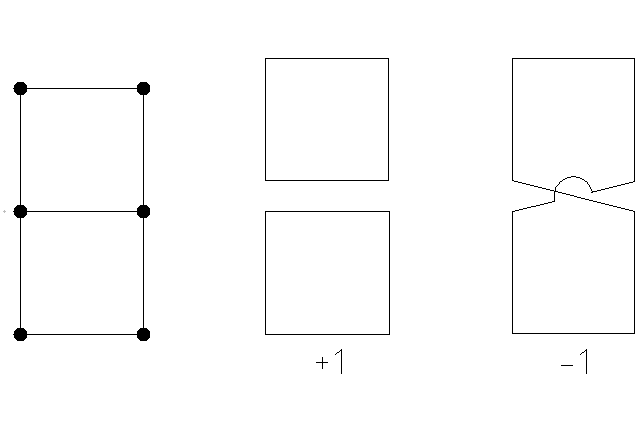
\includegraphics[width=0.7\columnwidth]{v2}
	\caption{Altro grafico ambiguo}
	\label{fig1}
	\end{figure}
\end{frame}

\begin{frame}
\frametitle{Generalizzazione del teorema di Gauss}
\begin{itemize}
\item<1->{Teorema di Gauss\\
Angolo spazzato dalla tangente di una curva piana \textbf{senza autointersezioni} è $2\pi$}
\item<2->{Si può generalizzare ad una curva \textbf{con autointersezioni} e vale $2(k+1)\pi$, con $k$ numero pesato dei nodi.
\begin{figure}[r]
	\centering
	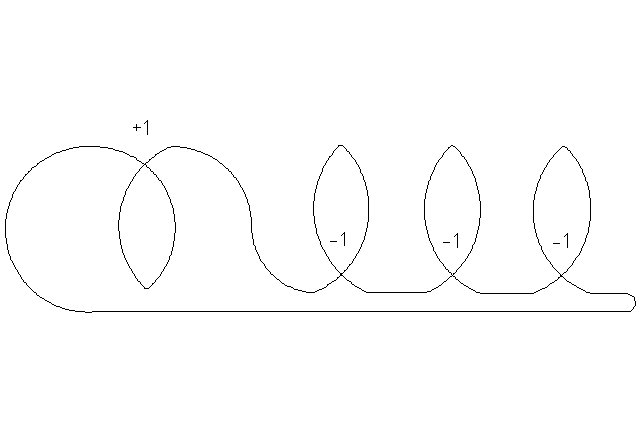
\includegraphics[width=0.7\columnwidth]{curva}
	\caption{L'angolo spazzato è $-2\pi$}
	\label{fig1}
	\end{figure}}
	\end{itemize}
\end{frame}
\begin{frame}
\frametitle{La definizione di maglia}
Ricordiamo che
\begin{itemize} 
\item{\textbf{maglia} $\to$ una sola poligonale chiusa}
\item{\textbf{grafico} $\to$ l'unione di una o più maglie disgiunte}
\end{itemize}
Perché questa definizione?\\
Non cerchamo direttamente il grafico di perimetro $r$ ma passiamo attraverso le maglie che lo compongono.\\
$f_r$ numero di maglie disegnabili con perimetro $r$ allora per i grafici composti da due maglie vale
$$g_r^{(2)}=\frac{1}{2!}\sum_{r_1+r_2=r}f_{r_1}f_{r_2}$$
\end{frame}
\begin{frame}
\frametitle{Grafici come unione di maglie}
Vogliamo combinare
\begin{itemize}
\item{quante maglie voglio $\to s$}
\item{di tutte le lunghezze possibili $\to r_1, r_2... r_s$}
\end{itemize}
$$
\Phi(v)=\sum_{s=1}(-1)^s\frac{1}{s!}\sum_{r_1,r_2,...=0}^\infty v^{r_1+r_2+...r_s}f_{r_1}...f_{r_s}
$$
Questa espressione si può manipolare e ottenere uno sviluppo in serie di un esponenziale nella forma

$$ \Phi(v)= \exp \left[ - \sum_{r=0}^\infty v^r f_r \right] $$
indicando con $r=r_1+r_2+...+r_s$ e con $f_r=f_{r_1}\times f_{r_2}\times...\times f_{r_s}$\\
\center{L'unica incognita è $f_r$, numero di maglie di lunghezza $r$.}
\end{frame}

\begin{frame}
\frametitle{Parametrizzazione delle poligonali}
Come ci si muove su un reticolo?
\begin{itemize}
\item<1->{Layout dell'informazione:
$$(i,j,\mu)$$
dove $i$, $j$ sono le coordinate del sito e $\mu$ indica la direzione \textbf{di ingresso} nel sito nel modo seguente \\

\begin{center}
\begin{tabular}{| c | c | c | c | c | }
  \hline                       
  $\mu$ & 1 & 2 & 3 & 4 \\ \hline
    direzione & $\rightarrow$ & $\downarrow$ & $\leftarrow$ & $\uparrow$ \\
  \hline  
\end{tabular}
\end{center}
}
\end{itemize}

\end{frame}

\begin{frame}
\frametitle{Parametrizzazione delle poligonali - Funzione W}
\begin{itemize}
\item{Date le condzioni iniziali $(i_0,j_0,\mu_0)$, definisco
$$W_r(i,j,\mu) =  \# \ pesato \ di \ cammini \ da \ (i_0,j_0,\mu_0) \ a \ (i,j,\mu) \ lunghi \ r
$$}
\item{Per chiudere i cammini basta chiedere
$$
W_r(i_0,j_0,\mu)
$$
e per definizione si torna al punto di partenza}
\end{itemize}

\end{frame}

\begin{frame}
\frametitle{Proprietà ricorsive di W}
Ovviamente la funzione $W$ gode di proprietà ricorsive
\begin{equation}
\begin{split}
&W_{r+1}(i,j,1)  = \\&W_r(i-1,j,1)+e^{-i\frac{\pi}{4}}W_r(i-1,j,2)+0+e^{i\frac{\pi}{4}}W_r(i-1,j,4) 
\end{split}
\end{equation}
\begin{figure}[h]
\centering
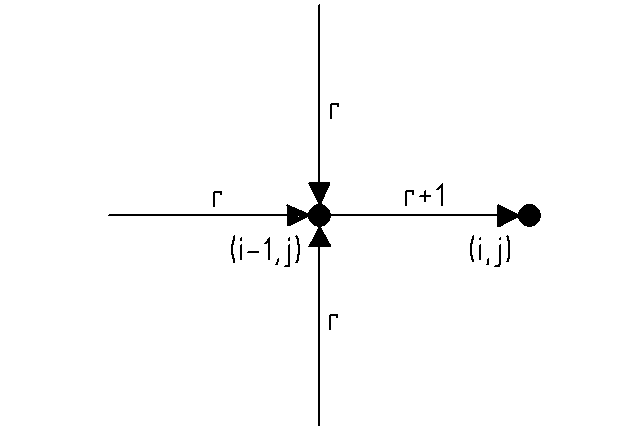
\includegraphics[width=0.7\columnwidth]{v7}
\caption{Rappresentazione grafica dell'equazione ricorsiva}
\label{v7}
\end{figure}
\end{frame}

\begin{frame}
\frametitle{La matrice $\Lambda$}
\begin{itemize}
\item{Ho molte equazioni ricorsive al variare di posizione e direzione}
\item{Sono tutte lineari}
\end{itemize}
Deduco che esiste una matrice $\Lambda$ tale per cui
$$
W_{r+1}(i,j,\mu)=\sum_{i',j',\mu'}\Lambda(ij\mu|i'j'\mu')W_{r}(i',j',\mu')
$$
che essendo ricorsiva diventa
$$
W_{r+1}(i,j,\mu)=\sum_{i_0,j_0,\mu_0}\Lambda^{r+1}(ij\mu|i_0j_0\mu_0)W_{0}(i_0,j_0,\mu_0)
$$
Notiamo che $\Lambda$ è una matrice di grandi dimensioni.
\end{frame}

\begin{frame}
\frametitle{Significato della matrice $\Lambda$}
La matrice $\Lambda$ è l'oggetto che mi permette di fare evolvere il sistema.\\
I suoi coefficienti
$$\Lambda^r(i,j,\mu|i_0,j_0,\mu_0)$$
mi dicono se è possibile (e se sì con che fase) andare da $(i_0,j_0,\mu_0)$ a $(i,j,\mu)$.\\

Ricordiamoci che la scelta di $\mu_0$ non cambia il percorso, possiamo sceglierla come vogliamo. Poniamo
$$
\mu_0=\mu
$$
\end{frame}

\begin{frame} 
\frametitle{Il significato di $\Tr\Lambda^r$}
Quindi la traccia di $\Lambda^r$
$$ \Tr{(\Lambda^r)}=\sum_{i_0,j_0,\mu} \Lambda^r(i_0,j_0,\mu|i_0,j_0,\mu)
$$
è, a meno di un prefattore $1/2r$, il numero di tutte le maglie di lunghezza $r$ che possiamo evidenziare sul reticolo.\\

$$f_r=\frac{1}{2r}\Tr{(\Lambda^r)}
$$
Come trovo $\Tr{(\Lambda^r)}$?
\end{frame}

\begin{frame}
\frametitle{La traccia è un invariante}
Essendo la traccia un invariante possiamo calcolarla nella base diagonale, e otteniamo
$$
f_r=\frac{1}{2r}\Tr{(\Lambda^r)}=\frac{1}{2r}\sum_a \lambda_a^r
$$
dove $\lambda_a$ autovalori di $\Lambda$, che sono le nostre nuove incognite.\\

\end{frame}

\begin{frame}
\frametitle{Implementazione degli autovalori}
Supponiamo di avere gli autovalori
$$ \Phi(v)= \exp \left[ - \sum_{r=0}^\infty v^r f_r \right] = \Exp \left [ -\frac{1}{2}\sum_i\sum_{r=1}^\infty\frac{1}{r}v^r\lambda_i^r \right ]$$
Si riconosce lo sviluppo in serie di un logaritmo nella variabile $(v\lambda_i)$
$$
\Phi(v) = \Exp \left [ \frac{1}{2} \sum_i \Log (1-v\lambda_i) \right]= \prod_i \sqrt{1-v\lambda_i}
$$
\end{frame}


\begin{frame}
\frametitle{Calcolo degli autovalori}
Potremmo dimostrare che
$$
\prod_i1-v\lambda_i=\Det(\textbf{1}-v\Lambda)=(1+v^2)^2-2v(1-v^2) \left( \cos{\frac{2\pi p}{L}}+\cos{\frac{2\pi q}{L}} \right)
$$
e sostituendo questa espressione nella funzione di partizione
\begin{equation}
\begin{split}
&Z_N(T)=\\
&=\left( \frac{1-v^2}{2}\right)^{-N}\prod_{p,q=0}^L \left[ (1+v^2)^2-2v(1-v^2) \left( \cos{\frac{2\pi p}{L}}+\cos{\frac{2\pi q}{L}} \right) \right]^{\frac{1}{2}}
\end{split}
\end{equation}

\end{frame}

\begin{frame}
\frametitle{Dalla funzione di partizione all'energia libera}
Ottenuta la funzione di partizione è sufficiente valutarne il logaritmo per ottenere l'energia libera
\begin{equation}
\begin{split}
&\frac{-F(T)}{kT}=\Log(Z_N)=\\
&=N\Log(2)-N\Log(1-v^2)+\\
&+\frac{1}{2} \sum_{p,q=0}^L\Log\left[ (1+v^2)^2-2v(1-v^2) \left( \cos{\frac{2\pi p}{L}}+\cos{\frac{2\pi q}{L}} \right) \right]
\end{split}
\end{equation}
\end{frame}

\begin{frame}
\frametitle{Limite termodinamico per F(T)}
Nel limite termodinamico in cui $L\to \infty$ otteniamo
\begin{equation}
\begin{split}
&\frac{-F(T)}{kT}=\\
&=N\Log(2)-N\Log(1-v^2)+
\\&+\frac{N}{2(2\pi)^2}\int_0^{2\pi} d\omega_1 d\omega_2 \Log\left[ (1+v^2)^2-2v(1-v^2) \left( \cos{\omega_1}+\cos{\omega_2} \right) \right]
\end{split}
\end{equation}
Notiamo che $F(T) \propto N$.\\
Nota l'energia libera si deriva la termodinamica, in particolare la \textbf{Temperatura di Curie}.
\end{frame}

\begin{frame}
\frametitle{Singolarità di $F(T)$}
Transizioni di fase $\to$ Singolarità di $F(T)$
\begin{equation}
\begin{split}
&\frac{-F(T)}{kT}=\\
&=N\Log(2)-N\Log(1-v^2)+
\\&+\frac{N}{2(2\pi)^2}\int_0^{2\pi} d\omega_1 d\omega_2 \Log\left[(1+v^2)^2-2v(1-v^2) \left( \cos{\omega_1}+\cos{\omega_2} \right) \right]
\end{split}
\end{equation}
\begin{itemize}
\item{Caso banale di $v=1 \ \to \ T=0$}
\item{Minimo dell'argomento del logaritmo $\to \cos\omega_1 = \cos\omega_2=1$. \\
Altre due singolarità $v_-$ e $v_+$.}
\end{itemize}
\end{frame}

\begin{frame}
\frametitle{Le soluzioni non banali $v_-$ e $v_+$}
Si cercano le radici del polinomio
\begin{equation}\label{poli}
(1+v^2)^2-4v(1-v^2)=(v^2+2v-1)^2
\end{equation}
e si ottengono
$$
\begin{cases} v_-=-(1+\sqrt{2}) & \to T_C = (0.166+0.590i)J/k  \\ v_+= -1+\sqrt{2}, & \to T_C=2.269 J/k
\end{cases}
$$

\begin{figure}[r]
	\centering
	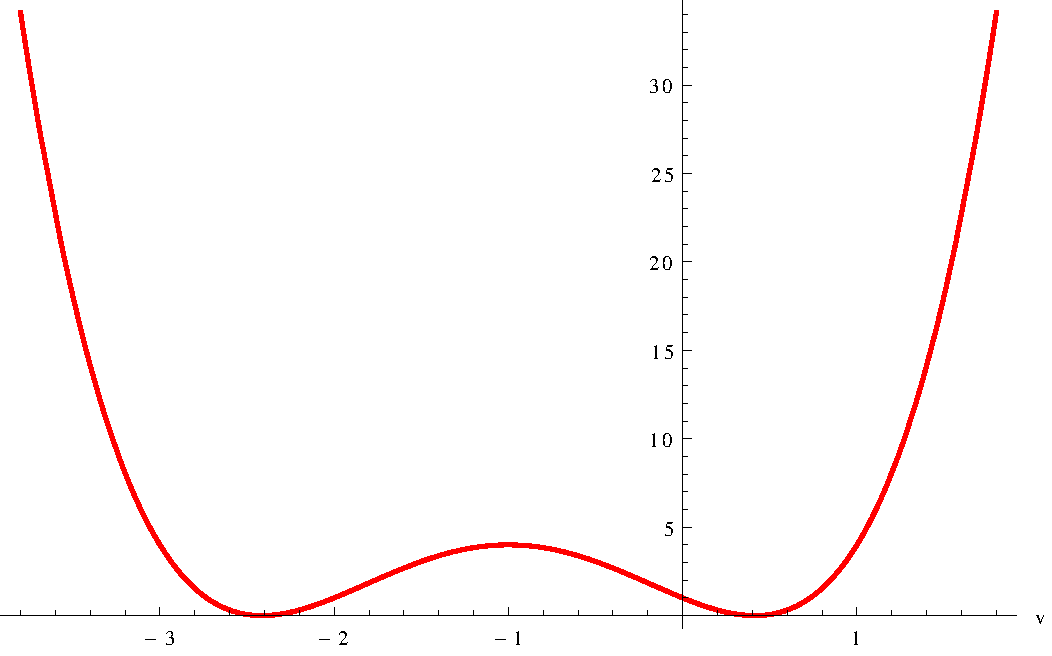
\includegraphics[width=0.5\columnwidth]{singo}
	\caption{Plot del polinomio (\ref{poli})}
	\label{fig1}
	\end{figure}

\end{frame}

\begin{frame}
\frametitle{Bibliografia}
\begin{itemize}
\item{Mussardo G., \emph{Il modello di Ising, introduzione alla teoria dei campi e delle transizioni di fase}, Bollati Boringhieri, Torino, pp 174-176, 198-204.}
\item{Ising E., \emph{Beitrag zur Theorie des
Ferro - und Paramagnetismus}, BIBLIOTHECA AUGUSTANA on line.}
\end{itemize}

\end{frame}






\end{document}
